\section{Introduction}

Thus far in the dissertation, I have used stimuli from the attraction and repulsion effect to explore perceptual and decisional processes in both perceptual and preferential choice. I showed that stimuli which are more similar to one another, and are thus more easily comparable, generate valuations with stronger correlations. This result holds across both perceptual choice (Chapter 2) and preferential choice (Chapter 4). I define the comparison process as a cognitive operation where a participant attends to the relative difference between two options on a choice set, typically (though not necessarily) on a single dimension. 

Embedded in a Thurstonian choice model \parencite{thurstone1927law}, these correlations can produce the repulsion effect \parencite{spektorWhenGoodLooks2018b,simonson2014vices} because the decoy option, whose value is tightly correlated with the target, occasionally exceeds the target in perceived value and thus "steals" choice shares from the target. 

In this chapter, I directly manipulate stimulus comparability in a perceptual choice task in an attempt to understand the relationship between comparability and choice. I first review previous literature on comparability and then present the results of a perceptual choice experiment.

\subsection{Previous Literature on Comparability}

Other researchers have studied the comparison process in decision-making, particularly in high-level choice (e.g., preferential). I first discuss the preferential choice work before transitioning to previous research on perceptual choice. 

\textcite{changWhichCompromiseOption2008} tested the compromise effect by varying the presentation of options. In the compromise effect, a “middle” ground option decreases the choice share of two dissimilar, “extreme” options. \textcite{changWhichCompromiseOption2008} displayed the options either by-alternative format, where option names are listed as columns while attribute values are listed as rows, or by-attribute, where option attributes are columns while option names are rows. The former display makes it more difficult to compare options on a single attribute, while the latter makes it easier. \textcite{changWhichCompromiseOption2008} found that listing options by-attribute increased the choice share of the compromise option, relative to a by-alternative display. 

\textcite{cataldoComparisonProcessAccount2019b} replicated this result, also finding that a by-alternative format nullified the attraction effect. The authors attributed this result to a “flexible comparison process”, where the comparison strategy is influenced by display format. According to this account, the by-attribute format increases the ease of target-decoy comparisons relative to the by-alternative format \footnote{\textcite{hasan2025registered} failed to replicate these results, albeit with slightly different decoy types.}. \textcite{cataldoReversingSimilarityEffect2018b} showed that presenting options in a format that encourages within-dimension comparisons on pairs of options can reverse the well-studied similarity effect.

\textcite{noguchi2014attraction} studied context effects using eye-tracking, showing that people tend to compare pairs of options on a single attribute, and that this appears to drive the attraction, similarity, and compromise effect. In their study, participants' eye movements showed that they were more likely to transition between options on a single dimension than they were to transition between dimensions within a single option. They also found that transitions between two options are negatively related to the choice share of a third option.

\textcite{hayes2024attribute} manipulated attribute comparability, such that the dimensions of each option were either measured in the same unit (high comparability, e.g., 0-10 ratings) or in different units (low comparability, e.g., CPU speed vs. RAM for laptops). They found that the attraction effect only occurred in the low comparability condition. 

\textcite{hasan2025registered} conducted a large scale replication of the attraction effect, systematically varying option order, presentation mode (numerical or graphical), and presentation format (by-attribute or by-alternative). They found that the attraction effect was stronger when the target and decoy options were adjacent to one another, presumably because this allows for easier target-decoy comparison. The attraction effect was stronger when attributes were presented numerically compared to graphically, a result found by other researchers \parencite{frederickLimitsAttraction2014b,yangMoreEvidenceChallenging2014}. They did, however, fail to replicate \textcite{cataldo}'s finding that the attraction effect varies with by-alternative vs. by-attribute format.

Hsee and colleagues \parencite{hseeEvaluabilityHypothesisExplanation1996,hseeLessBetterWhen1998,hseeWillProductsLook1998,hsee1999preference} have also shown that the comparison of options affects consumer behavior. For example, they repeatedly showed that participants’ evaluation of a given option can change with the addition of a reference point (i.e., lower valued options improve with a high reference point and vice versa). That is, participants’ judgments can reverse when options are evaluated jointly, compared to separately \parencite{hsee1999preference}. 

Many theoretical accounts of decision-making rely on the comparison process to account for context effects. According to \textcite{trueblood2014multiattribute}'s Multiattribute Linear Ballistic Accumulator Model (MLBA), each option accumulates evidence through pairwise comparisons to all other available options. This comparison is modulated by several processes, such as distance in attribute space and extremeness aversion. \textcite{roeMultialternativeDecisionField2001a}'s Multialternative Decision Field Theory (MDFT) model also assumes that options accumulate evidence through comparison, and that comparisons between nearby options exhibit greater influence on preference. Other decision models incorporate similar mechanisms \parencite{usherLossAversionInhibition2004a,noguchiMultialternativeDecisionSampling2018a,wollschlager2NaryChoiceTree2012a,landry2021pairwise} (c.f. \textcite{bhatiaAssociationsAccumulationPreference2013b,bergnerVAMPVotingAgent2019b}). 

\textcite{trueblood2022attentional} argued that options that are more similar garner more attention in the comparison process. They presented a simple Markov model where pairwise comparisons on a single attribute determine the accumulation of preference, and the time spent on a comparison is an increasing function of the similarity of options on the attribute. Their model can successfully, and simply, account for the "big three" context effects (attraction, repulsion, and similarity).

\subsection{Comparability Effects in Perceptual Choice}
There has been other research, albeit relatively limited, on the comparison process in perceptual decision-making. Much of this work has focused on the spatial layout of the options and its effect on perceptual context effects.

\textcite{trueblood2022attentional} re-analyzed previous perceptual choice context effect data \parencite{trueblood2015fragile} by examining the order of the options on the screen. They found that the attraction effect was strongest when the target and decoy were next to each other, while the effect was weak (or even nullified) when the options were separated spatially. Their conclusion, supported by a modeling analysis, was that people tend to compare pairs of options which are spatially closer to one another more often than pairs further away from one another. This result may seem obvious, but previous researchers have largely ignored the order of options in choice, generally collapsing over order in all analyses.

\textcite{evansImpactPresentationOrder2021} found a similar result in perceptual choice, though in their experiment the options were separated both spatially and temporally. In their experiment, participants saw three rectangles, presented sequentially, and selected the largest rectangle after all stimuli were presented. They found that orders in which the target and decoy were presented in the latter two positions elicited an attraction effect, whereas orders in which the competitor and decoy were presented in the latter two positions tended to elicit a repulsion effect. They interpreted their results as evidence that the comparison process can be altered through spatial and temporal properties of the stimuli.

Another interpretation of their results, and those of \textcite{trueblood2022attentional}, is that by altering the location and timing of the stimuli, the researchers are also altering the comparability. In the perceptual model of Chapter 2, increased comparability is represented by an increase in perceptual correlation. As shown previously, this perceptual correlation can create a repulsion effect by allowing the decoy to more easily "steal" choice shares from the target.

The experiments of \textcite{evansImpactPresentationOrder2021} and \textcite{trueblood2015fragile} are interesting and have to much to tell us about the role of comparability in decision-making. However, I wished to isolate the effect of comparability from context effects. To do so, I conducted an experiment where participants saw three rectangles at a time and selected the largest one. On critical trials, two of these rectangles were equally large but oriented differently (i.e., \textit{focal} rectangles, as in Experiments 1, 2, and 3). A third \textit{decoy} option was a square, and thus equally similar to either option. I designated one of the two focal options as the \textit{target} based on its proximity and comparability to the decoy. Based on the results of Chapter 2, this should increase the correlation between the comparable options and result in a \textit{decrease} in the target's choice share. These predictions are generally borne out in the data, albeit with limitations which will be adressed in future work.

\section{Experiment 5}
Experiment 5 adresses the effect of comparability in perceptual choice. To do so, I incorporated \textit{symmetrically dominated decoys}. A symmetrically dominated decoy is not only dominated by both focal options, but also equally similar to both options. Thus, the terms target and competitor, which have been used throughout this dissertation, take on a different meaning here. The target option is the option that is both adjacent to and easily comparable to the decoy.

\subsection{Methods}

\subsubsection{Participants}
$231$ undergraduate students at the University of Massachusetts Amherst participated in the lab, in exchange for course credit. $17$ participants' data were removed from all analyses becauses they failed to achieve at least $80\%$ correct on catch trials (see below), leaving final sample size of $N=214$. 

\subsubsection{Stimuli}
The stimuli were gray-scale rectangles and squares, varying systematically on height and width. 

The critical stimuli are depicted in Figure~\ref{fig:comparability_stim_plot}. The focal stimuli ($H$ and $W$) are equal in area and fell on two diagonals, the upper diagonal area being $25000$ square pixels and the lower diagonal being $7581$ square pixels. The decoy options were either $20\%$ or $35\%$ smaller than the focal options.

\begin{figure}
   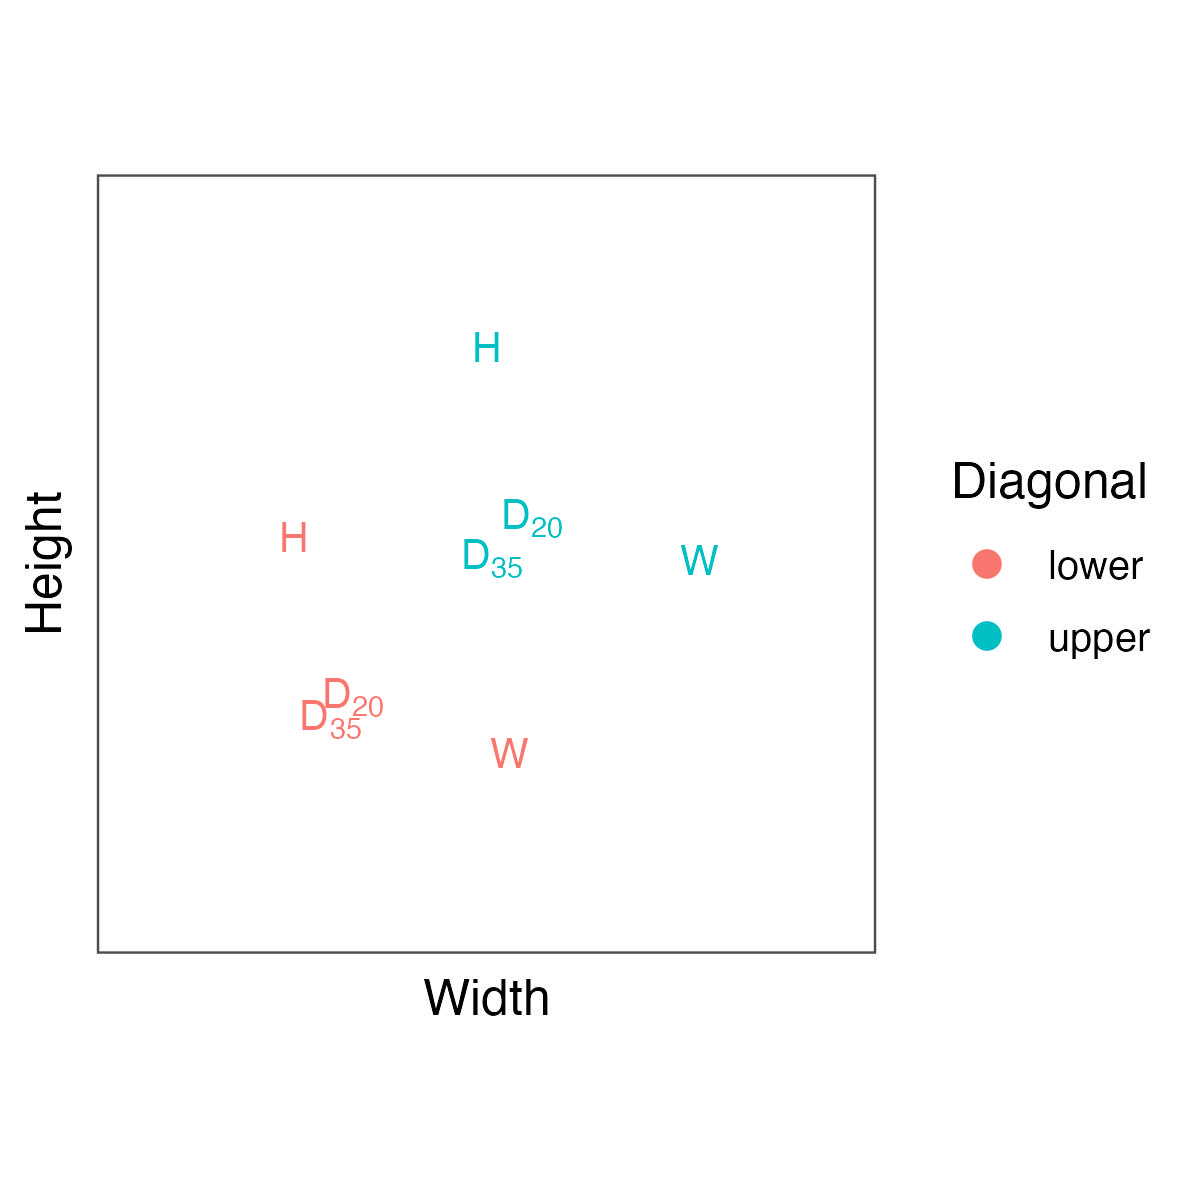
\includegraphics[width=100mm]{figures/comparability_stim.jpg}
   \caption{Graphical depiction of critical stimuli from Experiment 5. The stimuli fall on two diagonals, labeled as upper and lower. The H rectangles are taller than wide, while the W rectangles are wider than tall. The decoy (D) rectangles are equally wide and tall (i.e., squares), and the subscripts indicate the $TDD$ value.}
   \label{fig:comparability_stim_plot}
\end{figure}

There were other types of stimuli on non-critical trials, which are explained below.

\subsubsection{Design}
Trials were split into four blocks in the experiment.

There were four types of trials: critical trials, filler-square trials, filler-random trials, and catch trials.

On each critical trial, there were three options: an $H$ rectangle, a $W$ rectangle, and a $D$ rectangle. The focal rectangles fell on two diagonals (upper and lower, see above), while the decoy rectangle varied in $TDD$ at $20\%$ and $35\%$. 

The stimuli were arranged in one of four displays: all-aligned, two-aligned, none-aligned, or triangle. See Figure~\ref{fig:comparability_trials} for sample trials. 

In the all-aligned display, all stimuli were arranged in a horizontal array, as in the experiments of \textcircled{trueblood2013not} and \textcite{spektorWhenGoodLooks2018b} (Experiment 4). 

In the two-aligned display, two options were aligned horizontally in the top-left and top-middle positions, while the third option was placed in the bottom-right position of the screen. This is a crucial condition and an instantiation of the "comparability" hypothesis, in which the comparison of the two aligned options is far easier than all other pairwise comparisons.

In the none-aligned display, all options are located in different vertical and horizontal positions, such that all comparisons should (in principle) be more difficult.

The triangle display is identical to the triangle display of Experiments 1 and 2, with the exception that on half of all triangle display trials, the triangle was inverted.

In all displays, the horizontal distances between all options was constant.

\begin{figure}
   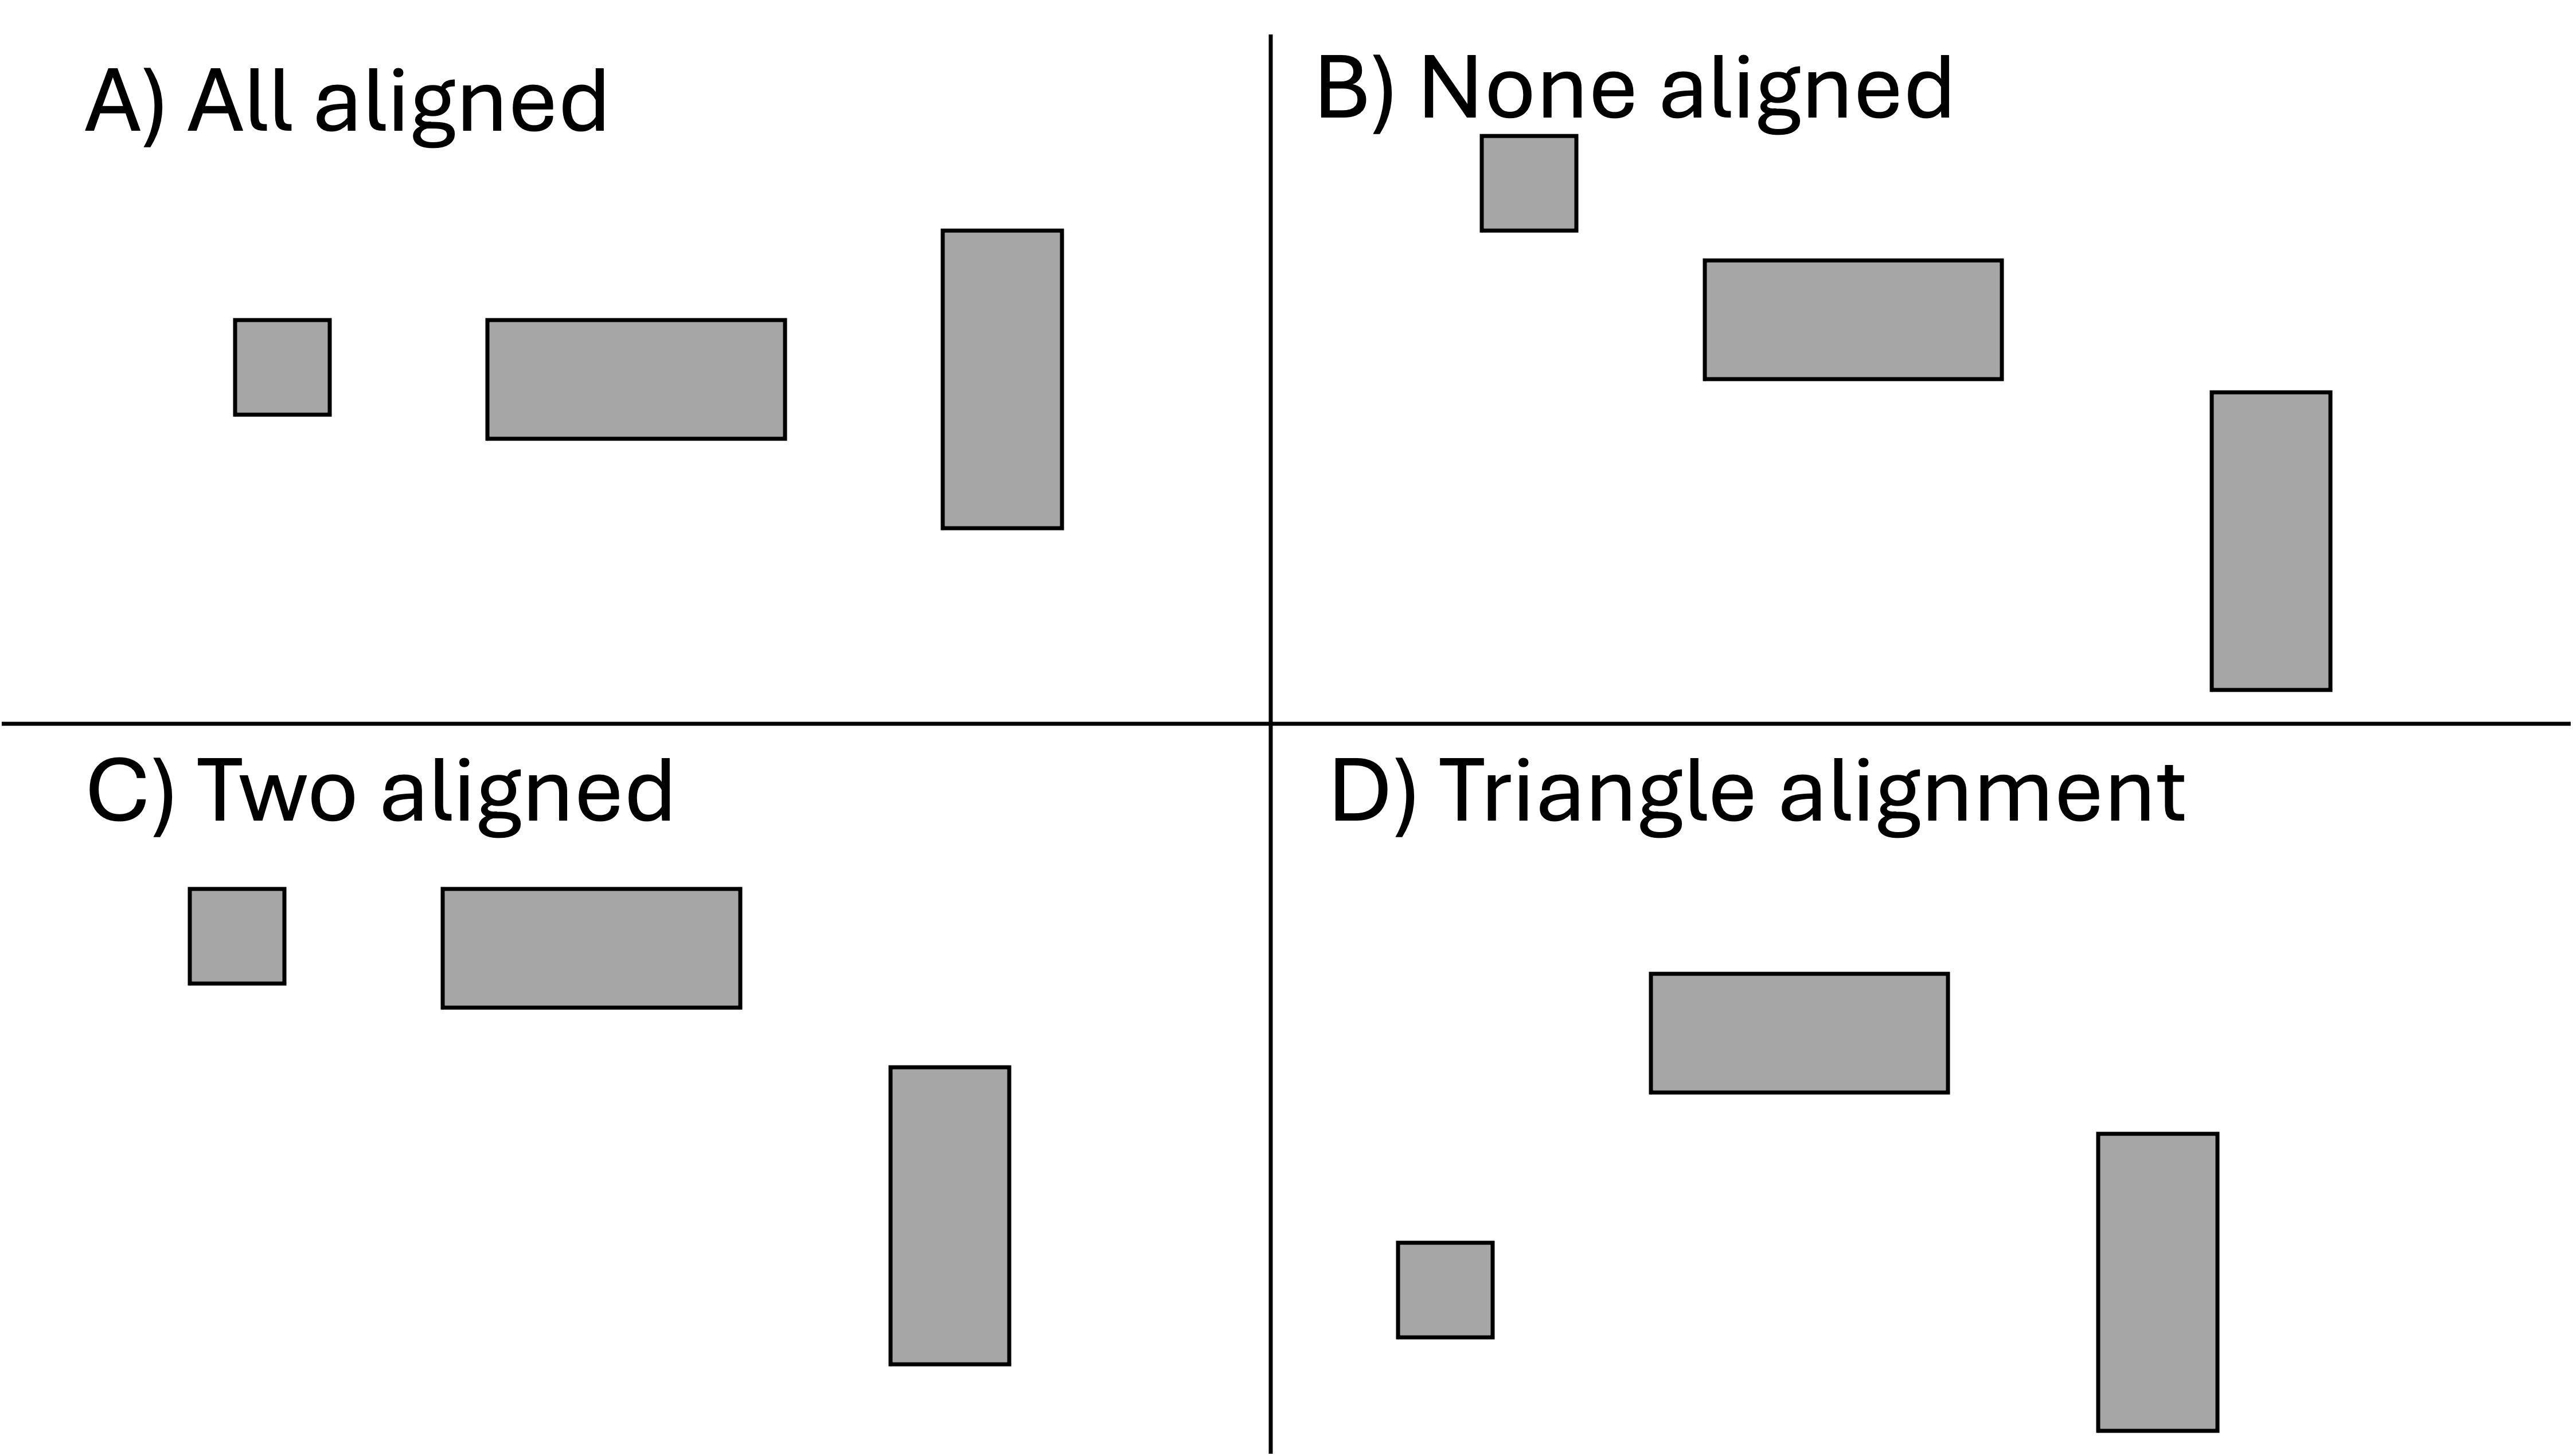
\includegraphics[width=100mm]{figures/comparability_design.jpg}
   \caption{Critical trials from Experiment 5.}
   \label{fig:comparability_trials}
\end{figure}

In addition to varying diagonal, $TDD$, and display, I also varied option order, such that all six orders ($DHW$, $DWH$, $HDW$, $HWD$, $WDH$, and $WHD$) were equally common.

This was a $2$ (diagonal: lower, upper) x $2$ ($TDD$: $20\%$, $35\%$) x $4$ display: (all-aligned, two-aligned, none-aligned, triangle) x $6$ (order: $DHW$, $DWH$, $HDW$, $HWD$, $WDH$, and $WHD$) within-participants study. Each participant completed $4$ trials for all combinations of these factors ($1$ per each of the four blocks), except for the two-aligned trials, for which they completed $8$ trials ($2$ per each of the four blocks). Thus, there were a total of $480$ critical trials ($(2*2*3*6*4)+ (2*2*1*6*8)=480$).

On filler-random trials, three options were randomly generated by sampling a height and width from the $U(57,200)px$ distribution. There were $40$ filler-random trials per block for each of four blocks, leading to a total of $160$ filler-random trials. 

On filler-square trials, a square was randomly generated by sampling a side length from the $U(57,200)px$ distribution. Then, two non-square rectangles were generated by sampling a height and width from a the $U(57,S)px$ distribution, where $S$ is the side length for the square. This ensured that the square was always the largest option on these trials. These trials were included to ensure that participants did not learn to ignore the squares, as the critical trials rely on participants comparing the squares to the focal options. There were $40$ filler-square trials per block for each of four blocks, leading to a total of $160$ filler-square trials.

On catch trials, one large option was randomly generated by randomly sampling a stimulus from the upper diagonal (see Figure~\ref{fig:comparability_stim_plot}), and two smaller options were randomly sampled from the lower diagonal. Here, one option was always much larger than the other two, allowing me to remove participants who did not perform poorly. There were $10$ catch trials per block for each of four blocks, leading to a total of $40$ catch trials.

On each of the non-critical trials, stimulus order was randomized. Additionally, one of the four displays (all-aligned, two-aligned, none-aligned, triangle) was selected at random.

There were a total of $840$ trials in the experiment ($480$ critical + $160$ filler-random + $160$ filler-square + $40$ catch=$840$).

\subsubsection{Procedure}
On each trial, participants saw three rectangles, labeled '1', '2', and '3'. They selected the largest rectangle by pressing the corresponding key on the keyboard. 

Trials were split into four blocks, with a 15-second break in between blocks.

\subsection{Results}

\subsubsection{Data Processing}
In addition to removing participants who failed to meet the $80\%$ correct criterion for catch trials, I removed all trials with RTs $<100ms$ or $>10,000ms$. 

\subsubsection{Catch and Filler Trials}
Participants performed well on the non-critical trials. On average, all participants performed above chance on the catch, filler-random, and filler-square trials, including on all display types. See Figure~\ref{fig:comparability_non_crit_mean_prop_correct} for data.

\begin{figure}
   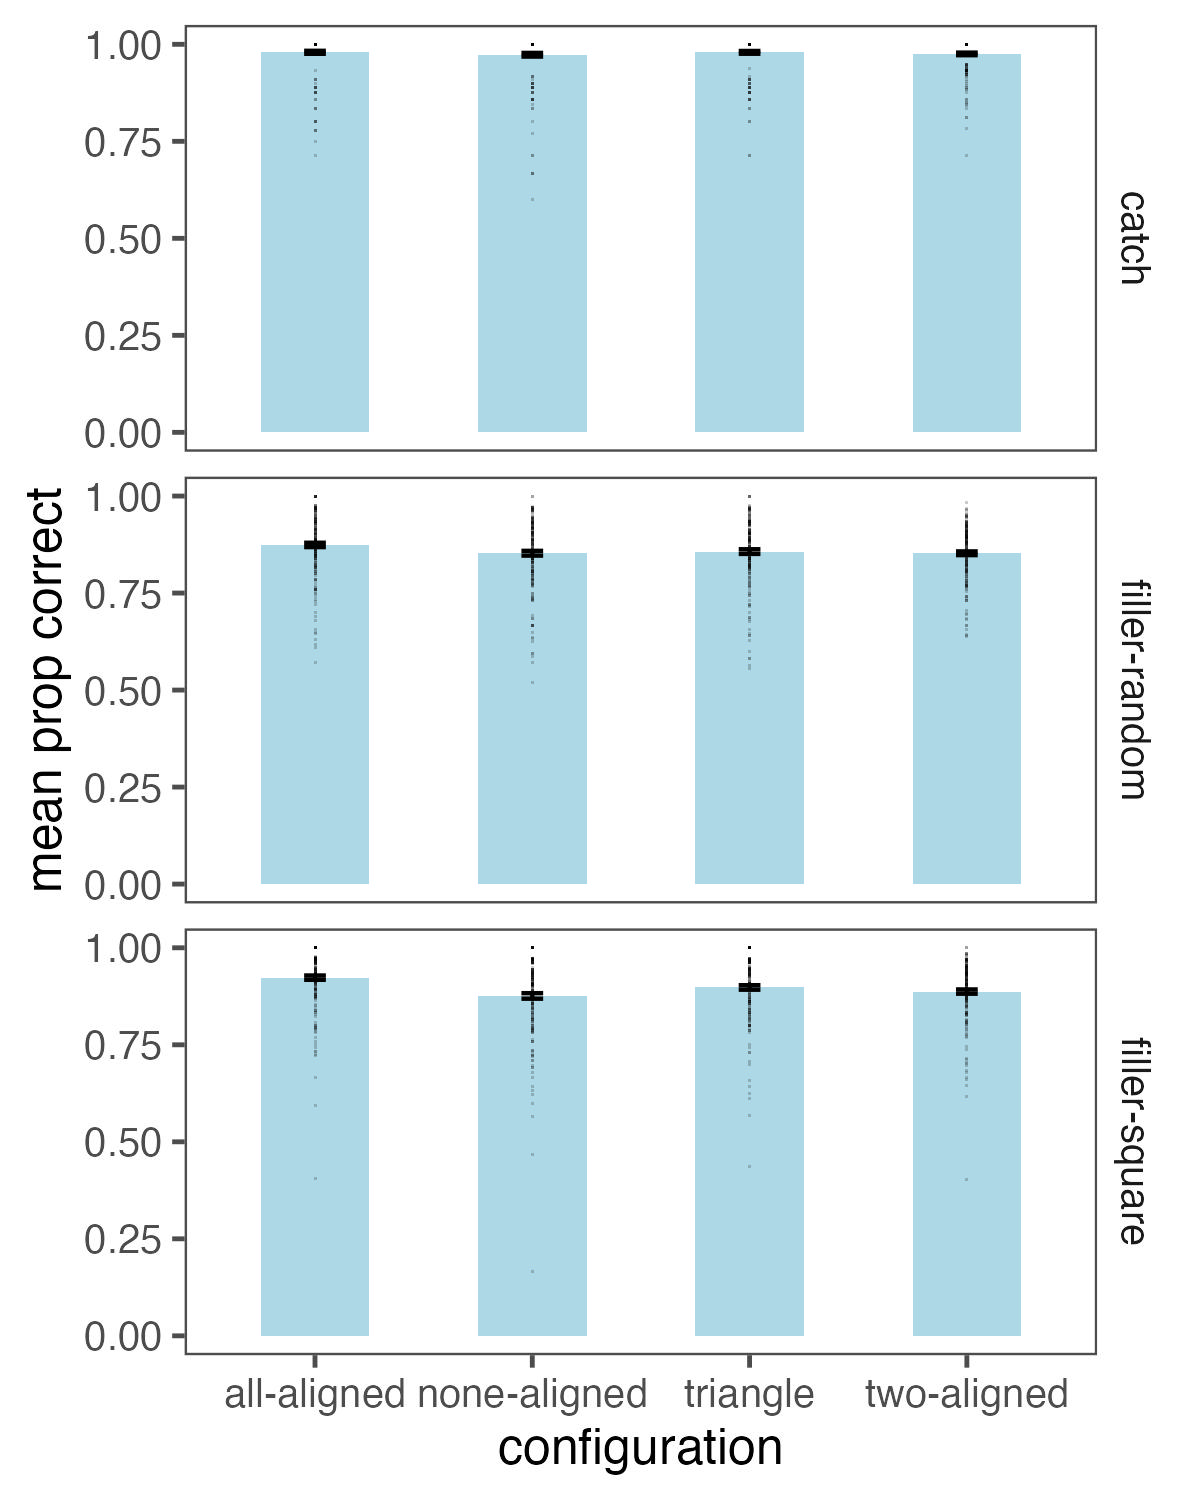
\includegraphics[width=100mm]{figures/comparability_non_crit_mean_prop_correct.jpeg}
   \caption{Results from non-critical trials in Experiment 4. Rows show trial types. Bars show mean proportion correct in a given condition, with the error bars showing $\pm1\text{SE}$. Dots show individual participant data.}
   \label{fig:comparability_non_crit_mean_prop_correct}
\end{figure}

\subsubsection{Critical Trials}